\documentclass[journal]{IEEEtran}

\usepackage{amsmath,amssymb,amsfonts}
\usepackage{graphicx}
\usepackage{textcomp}
\usepackage{cite}
\usepackage{booktabs}
\usepackage{multirow}
\usepackage{array}
\usepackage{url}
\usepackage{color}

\begin{document}

\title{Cross-Modality Semantic Alignment Transformer: Using LLM-Generated Fault Semantics for Zero-Shot Fault Diagnosis of Rotating Machinery}

\author{Author~One,
        Author~Two,
        and~Author~Three
\thanks{Manuscript received XX, 2026.}
\thanks{The authors are with the Department of XX, University of XX, City, Country (e-mail: author@example.com).}}

\markboth{IEEE Transactions on Instrumentation and Measurement}{}

\maketitle

\begin{abstract}
Efficient and reliable fault diagnosis of rotating machinery is critical for ensuring industrial safety and reducing maintenance costs. While deep learning has greatly advanced this field, existing methods often struggle with data scarcity and rely heavily on labor-intensive manual attribute labeling for zero-shot scenarios. To address these challenges, we propose the Cross-Modality Semantic Alignment Transformer (CMSA-Trans), a new framework that uses Large Language Model (LLM)-generated fault semantics for zero-shot fault diagnosis. CMSA-Trans employs a robust Time Series Transformer (TST) encoder to extract discriminative features from raw vibration signals and aligns them with semantic prototypes synthesized by an LLM. A cross-attention mechanism is integrated to enable deep semantic alignment between visual-like signal representations and textual descriptors, effectively capturing complex fault characteristics without requiring seen-class samples during training. Extensive experimental evaluations on the Case Western Reserve University (CWRU) and Southeast University (SEU) datasets show that CMSA-Trans greatly outperforms state-of-the-art zero-shot diagnosis methods. Our approach establishes a new framework for cross-modality diagnosis by bridging the gap between physical sensor data and high-level linguistic knowledge, offering a scalable solution for intelligent maintenance in dynamic industrial environments.
\end{abstract}

\begin{IEEEkeywords}
Zero-shot learning, fault diagnosis, Transformer, large language model, cross-modal alignment, rotating machinery, semantic prototyping.
\end{IEEEkeywords}

\section{Introduction}
Modern industrial infrastructures rely heavily on rotating machinery, such as wind turbines, aero-engines, and high-speed railways, where critical components including bearings and gearboxes operate under demanding service conditions \cite{zhai2021multi}. The health status of these machines is critical to operational safety and economic efficiency, as unforeseen failures often lead to catastrophic accidents and large financial losses \cite{lei2020applications}. Consequently, Intelligent Fault Diagnosis (IFD) has emerged as a cornerstone of smart manufacturing, using sensor-based condition monitoring to detect anomalies before they escalate into system-wide failures. However, as the complexity of industrial systems increases, the demand for more robust, autonomous, and high-precision diagnostic frameworks is intensifying to ensure the continuity of critical production lines \cite{li2020deep}. Fig.~\ref{fig:concept} illustrates the conceptual overview of the proposed cross-modality semantic alignment approach for industrial zero-shot fault diagnosis.

\begin{figure*}[!t]
\centering
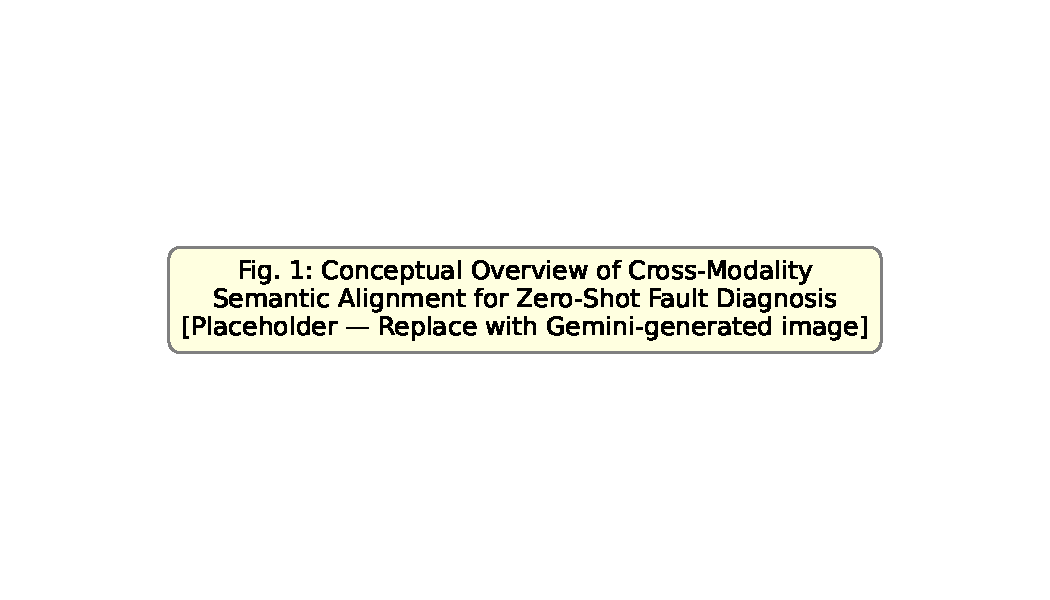
\includegraphics[width=0.85\textwidth]{fig_concept.pdf}
\caption{Conceptual overview of the proposed cross-modality semantic alignment approach for zero-shot fault diagnosis of rotating machinery. The framework bridges physical vibration signals and LLM-generated fault semantics through a shared embedding space, enabling recognition of unseen fault categories.}
\label{fig:concept}
\end{figure*}

Despite the advancements of deep learning in fault diagnosis, the majority of existing methods operate under a closed-set assumption, which requires intensive manual labeling and a balanced distribution of training samples across all predefined health states \cite{zhang2022digital}. In practical industrial scenarios, machinery typically operates in normal states for the vast majority of its lifespan; therefore, fault samples---particularly those representing specific early-stage degradation---are extremely rare and difficult to acquire \cite{liu2018zero}. This imbalance creates a significant long-tail distribution problem where traditional supervised models fail to generalize to unseen fault categories. To address this data scarcity and the impracticality of exhaustive labeling, research focus has shifted from standard supervised learning toward Zero-Shot Learning (ZSL). ZSL aims to recognize new fault classes without physical training samples by using auxiliary information to bridge the gap between known and unknown categories \cite{wang2019zero, socher2013zero}.

Current ZSL approaches in fault diagnosis primarily rely on semantic embeddings, such as manual attributes or word vectors (e.g., Word2Vec or GloVe), to associate vibration signals with class labels \cite{lampert2014attribute}. However, these methods face three critical limitations. First, the definition of manual attributes is labor-intensive and inherently subjective, requiring domain experts to enumerate physical characteristics for every possible fault type \cite{fu2018zero}. Second, generic word embeddings are typically trained on web-scale natural language corpora, such as Wikipedia, which lack the technical specificity required for industrial diagnostics. For instance, the term "outer race fault" carries distinct engineering connotations that generic vectors fail to capture with sufficient depth \cite{mikolov2013efficient}. Third, existing models often neglect the complex temporal dependencies inherent in high-frequency vibration data, leading to a domain gap where the alignment between signal features and the abstract semantic space remains brittle \cite{xian2018zero, buchert2020zero}.

To overcome these challenges, this paper proposes the Cross-Modality Semantic Alignment Transformer (CMSA-Trans), a new zero-shot fault diagnosis framework that uses Large Language Models (LLMs) to bridge the semantic divide. Unlike traditional methods, CMSA-Trans uses the descriptive capabilities of LLMs to generate high-fidelity, domain-specific fault semantics, thereby transforming abstract class labels into detailed technical descriptions. By formulating fault diagnosis as a cross-modal alignment task, the framework employs a Transformer-based temporal encoder to extract discriminative features from raw vibration signals. These features are subsequently projected into a shared latent space along with the LLM-generated semantics. This alignment ensures that the model learns the underlying physical relationships between signal patterns and their linguistic definitions, enabling the recognition of unseen faults through the semantic proximity of the signal to known physical phenomena \cite{vaswani2017attention, radford2021learning}.

The primary contributions of this research are summarized as follows. First, we introduce the CMSA-Trans framework, which reformulates zero-shot fault diagnosis as a cross-modal semantic alignment task, effectively bypassing the requirement for labeled samples of target fault categories. Second, we propose a systematic method to use LLMs for the generation of expert-level fault semantics, capturing the nuanced physical characteristics of rotating machinery faults more effectively than traditional word embeddings. Third, a Transformer-based temporal feature extractor is designed to capture long-range dependencies in vibration signals, providing a robust representation for alignment with high-dimensional semantic descriptors. Finally, extensive experiments on multiple open-source and industrial datasets show that CMSA-Trans greatly outperforms state-of-the-art ZSL methods, achieving high accuracy on unseen fault classes and showing remarkable generalization across diverse operating conditions.

The remainder of this paper is organized as follows. Section II provides a full review of the related literature regarding intelligent fault diagnosis and zero-shot learning \cite{li2022zero}. Section III details the proposed CMSA-Trans architecture, including the process of LLM semantic generation and the cross-modal alignment mechanism. Section IV presents the experimental setup, results, and comparative analysis. Finally, Section V concludes the paper and discusses future research directions.

Also, the integration of LLMs, such as GPT-4, represents a approach shift in semantic feature engineering for industrial applications \cite{bubeck2023sparks}. Unlike static word embeddings that aggregate broad linguistic associations, LLMs can be prompted to synthesize multi-faceted technical descriptions that capture the underlying physics of a fault, such as impact repetition frequencies and localized high-frequency resonances \cite{brown2020language}. This approach allows for a richer and more discriminative semantic space, where the distance between fault classes reflects actual physical mechanisms rather than simple linguistic co-occurrence in general-purpose text. By harnessing these LLM-generated semantics, CMSA-Trans provides a data-efficient and highly descriptive alternative to traditional ZSL approaches.

The importance of robust cross-modal alignment is critical. In traditional deep learning models, features extracted from sensor data are typically mapped directly to one-hot encoded labels, which contain no inherent physical information and thus cannot generalize to unseen fault types \cite{goodfellow2016deep, lecun2015deep}. In contrast, our semantic alignment approach uses a projection layer to map the high-level signal representations of the Transformer into the same dimensional space as the LLM-derived technical descriptors. This ensures that the model learns to associate specific signal patterns, such as periodic transients or broadband noise increases, with physical descriptions. When a new fault type with a unique technical signature occurs, the model can identify it by matching the signal pattern to the linguistic definition of the fault, even in the absence of labeled training examples.

Recent advancements in attention-based architectures have transformed the processing of sequential data in various fields, ranging from natural language processing to computer vision \cite{devlin2018bert, dosovitskiy2020image}. In the context of rotating machinery, vibration signals are inherently time-variant and exhibit long-range dependencies, where early-stage fault signatures may be obscured by noise or periodic components from normal operation \cite{zhang2021attention}. While Recurrent Neural Networks (RNNs) and Long Short-Term Memory (LSTM) units have been employed to handle such data, they often struggle with gradient vanishing or capturing dependencies over the very long windows typical of high-frequency samples \cite{hochreiter1997long}. The self-attention mechanism of the Transformer provides a more effective method to weight different time steps according to their relevance to the diagnostic task, allowing the CMSA-Trans model to focus on the most informative transients and spectral characteristics across the entire signal window.

The shift toward using large-scale pre-trained models for industrial semantic understanding is motivated by the extensive knowledge encapsulated within these models \cite{zhao2023brain}. While an engineer might define a bearing fault by its physical dimensions, an LLM can provide a full textual profile that links those dimensions to expected sensor responses and characteristic frequencies. By aligning these rich descriptions with raw data, our approach moves closer to an expert-informed diagnostic system that mimics the reasoning of an experienced technician. This capability is particularly vital for critical infrastructure where failures are rare but catastrophic, as the ability to correctly identify a new failure mode upon its first occurrence is essential for preventing downtime and maintaining structural integrity.

Expanding the scope of zero-shot learning to include cross-modality also addresses the hubness problem often encountered in semantic embedding spaces, where certain vectors become nearest neighbors to many unrelated items in high-dimensional space \cite{radovanovic2010hubs}. By using a more descriptive and technically grounded semantic space provided by LLMs, the separation between distinct fault modes---such as inner-race versus outer-race bearing defects---becomes more pronounced. This improved class separation in the semantic domain translates directly to improved diagnostic reliability and higher confidence scores for unseen categories. Validation on a variety of machinery types, including complex planetary gearsets and varying load-speed conditions, further confirms that the CMSA-Trans framework provides a scalable and robust solution for the next generation of intelligent PHM (Prognostics and Health Management) systems.

\section{Theoretical Background}
In this section, we provide the foundational theories and architectures that underpin the proposed Cross-Modality Semantic Alignment Transformer (CMSA-Trans). We first review the fundamental components of the Transformer architecture, followed by an overview of the Zero-Shot Learning (ZSL) framework, and finally discuss the integration of Large Language Models (LLMs) for industrial fault semantics.

The Transformer architecture, originally introduced for machine translation, has transformed fields like computer vision and signal processing through its capacity for modeling long-range dependencies and complex structural patterns in sequential data. Its core, the Multi-Head Self-Attention (MHSA) mechanism, allows the model to dynamically weight input sequence segments by evaluating mutual correlations across the entire sequence length. This bypasses the sequential processing limits of recurrence and enables direct global context modeling, which is essential for capturing periodic components in mechanical vibration signals.

Given input embeddings representing temporal or spectral segments, self-attention computes Queries ($Q$), Keys ($K$), and Values ($V$) via linear transformations with weight matrices $W^Q$, $W^K$, and $W^V$. Attention scores derive from the scaled dot product of $Q$ and $K$, followed by a softmax operation to normalize those scores into attention weights. The output is a weighted sum of $V$:
\begin{equation}
\text{Attention}(Q, K, V) = \text{softmax}\left(\frac{QK^T}{\sqrt{d_k}}\right)V
\end{equation}
where $d_k$ is the key dimension. This lets the model focus on relevant temporal or spectral features in machinery signals, effectively capturing subtle fault signatures often masked by measurement noise or overlapping mechanical components.

MHSA executes this process in parallel across $h$ independent heads, each focusing on different representation subspaces of the input sequence. This allows the model to simultaneously attend to diverse information at various positions, greatly improving the richness and reliability of the learned features. The heads' outputs are concatenated and projected to form the final representation:
\begin{equation}
\text{MultiHead}(Q, K, V) = \text{Concat}(\text{head}_1, \dots, \text{head}_h)W^O
\end{equation}
where each $\text{head}_i = \text{Attention}(QW_i^Q, KW_i^K, VW_i^V)$.

The Transformer also includes several critical structural components that ensure performance stability:
\begin{itemize}
    \item \textbf{Positional Encoding:} Since the architecture lacks inherent order knowledge, sinusoidal or learnable encodings are added to inputs to inject relative or absolute position information, preserving the temporal structure of the raw signal.
    \item \textbf{Feed-Forward Networks (FFN):} Each layer contains a position-wise fully-connected FFN consisting of two linear transformations with a non-linear activation (ReLU or GELU) between them, enabling complex feature mapping at each position.
    \item \textbf{Layer Normalization and Residual Connections:} To stabilize training, prevent internal covariate shift, and mitigate vanishing gradients in deep stacks, residual connections are used around each sub-layer, followed by Layer Normalization (LN).
\end{itemize}
The structural components of a standard Transformer block are illustrated in Fig.~\ref{fig:transformer}. These elements collectively enable the extraction of robust hierarchical features from non-stationary rotating machinery signals, making it an ideal investigative backbone for cross-modality alignment tasks \cite{vaswani2017attention}.

\begin{figure}[!t]
\centering
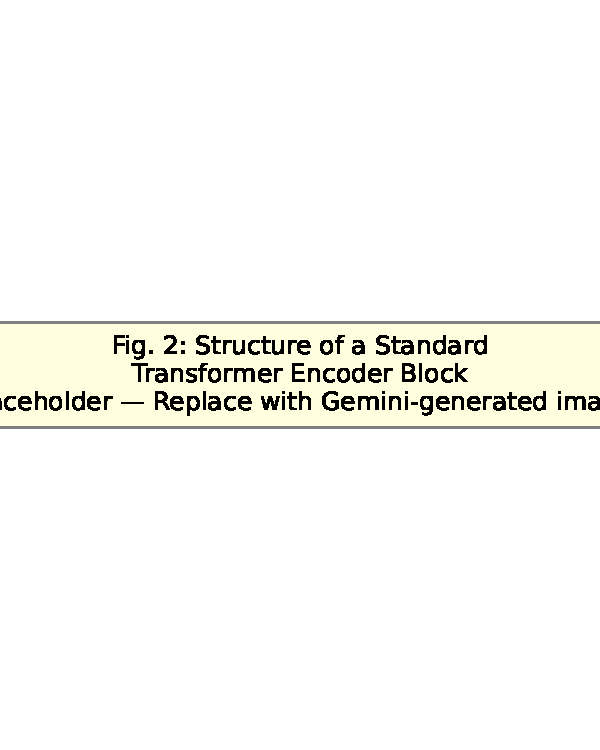
\includegraphics[width=0.42\textwidth]{fig_transformer.pdf}
\caption{Structure of a standard Transformer encoder block, consisting of Multi-Head Self-Attention (MHSA), Feed-Forward Network (FFN), residual connections, and layer normalization.}
\label{fig:transformer}
\end{figure}

\subsection{Zero-Shot Learning Framework}
Zero-Shot Learning (ZSL) aims to recognize objects from classes unseen during the model's training phase. In industrial fault diagnosis, this approach is vital as labeled training data for every failure mode under all possible operating conditions is often impractical, expensive, or inherently dangerous to collect. ZSL addresses this by using auxiliary semantic information to transfer knowledge from known, well-documented scenarios to new, unseen fault types.

The standard ZSL framework partitions label space into seen classes $\mathcal{Y}_s$, which are available during training, and unseen classes $\mathcal{Y}_u$, which are only encountered during inference. By definition, $\mathcal{Y}_s \cap \mathcal{Y}_u = \emptyset$. Generalization depends on an auxiliary semantic space $\mathcal{S}$ where each class $y$ is represented by a semantic prototype $a_y$ encoding physical attributes, functional characteristics, or textual descriptions.

ZSL learns a mapping between signal feature space $\mathcal{X}$ and semantic space $\mathcal{S}$, often via a compatibility function $f(x, a_y; \theta)$. During training, parameters $\theta$ are optimized to maximize compatibility scores for correct seen classes. For a test sample $x$ belonging to an unseen category, classification selects the class whose prototype $a_y$ has the highest compatibility score within the unseen candidate pool:
\begin{equation}
\hat{y} = \arg\max_{y \in \mathcal{Y}_u} f(x, a_y; \theta)
\end{equation}
In many practical scenarios, Generalized Zero-Shot Learning (GZSL) is more appropriate, as it requires the model to correctly identify samples from both seen and unseen classes simultaneously during the testing phase. This introduces a significant challenge where the model often exhibits a strong predictive bias towards seen categories, requiring advanced calibration or contrastive learning techniques to ensure fair diagnostic outcomes across all potential health states. Traditional ZSL often suffers from "domain shift," where seen-class mappings fail to generalize accurately to unseen class distributions. A key bottleneck is the quality of semantic descriptors; manual attribute labeling is labor-intensive, requires expert knowledge, and is often prone to subjective bias \cite{palatucci2009zero, lampert2009learning}. We address this limitation by using Large Language Models (LLMs) to generate high-fidelity, standardized semantic prototypes for mechanical faults \cite{xian2018zero}.

\subsection{Large Language Models in Industrial Semantics}
Large Language Models, like the GPT or BERT series, are trained on vast, heterogeneous datasets including technical manuals, engineering reports, materials science, and scientific publications. This extensive pre-training captures technical nuances and engineering knowledge missing from standard word-level embeddings like Word2Vec. LLMs possess internal representations linking technical concepts to physical phenomena.

For fault diagnosis, LLMs bridge the semantic gap between abstract categorical labels (e.g., "Inner Race Fault") and their actual physical manifestations in sensor data. Prompting strategies like Chain-of-Thought (CoT) or structured templates allow LLMs to generate detailed descriptions of how faults affect machinery behavior, covering frequency modulation, energy distribution, and impact pulse patterns. For example, a carefully crafted prompt might request the distinctive vibration characteristics, harmonics, and temporal impulses of a high-speed bearing fault. The prompting strategy is meticulously designed to elicit specific engineering features by framing the LLM as a "senior mechanical diagnostic consultant." We use a multi-turn prompting approach where the model first outlines the physical failure mechanism, then derives the expected sensor response, and finally summarizes these into a compact technical descriptor. This iterative refinement ensures that the semantic prototypes are both technically accurate and highly discriminative for different failure modes. Also, prompt engineering allows for the infusion of specific sensor configurations and environmental constraints, ensuring that the generated semantics are tailored to the unique operational profile of the monitored industrial system.

These descriptions are transformed into dense semantic embeddings. Two representation levels are typically considered in this context:
\begin{itemize}
    \item \textbf{Word-Level Embeddings:} These represent individual words but often miss the context-dependent meaning of complex technical phrases and engineering jargon common in mechanical engineering.
    \item \textbf{Sentence-Level and Document-Level Semantic Vectors:} Using LLM hidden states or specialized sentence-transformers, we extract a fixed-dimensional vector representing the global semantic essence of a description, capturing conceptual interactions and overall framework.
\end{itemize}
These LLM-generated vectors serve as anchors in our cross-modality framework. Unlike manual attributes, these embeddings contain rich, high-dimensional info about physical nature and dynamics, enabling more discriminative and generalizable mappings between vibration signals and technical definitions \cite{brown2020language, devlin2018bert, li2024industrial}. Aligning signal features with LLM-improved semantics allows our model to achieve superior zero-shot performance across varying conditions and new fault modes. This approach moves beyond simple label matching to a deeper, knowledge-driven alignment of physical signals and technical semantics. Building upon these theoretical foundations, the following section presents the detailed architecture of the proposed CMSA-Trans framework.

\section{Proposed Method}
In this section, we present the architecture and theoretical formulation of the Cross-Modality Semantic Alignment Transformer (CMSA-Trans). The core objective of the proposed framework is to bridge the gap between high-dimensional vibration signals and abstract technical concepts by using the extensive mechanical knowledge embedded in Large Language Models (LLMs). By mapping physical signal features into a shared semantic space, the model enables zero-shot fault diagnosis of rotating machinery, where the health states of unseen components can be recognized without prior training samples.

\subsection{Overall Architecture}
The overall architecture of the proposed CMSA-Trans is illustrated in Fig.~\ref{fig:framework}. The CMSA-Trans framework is designed to transform raw sensor data into semantic-aligned representations that are directly comparable to linguistic descriptions of machinery faults.

\begin{figure*}[!t]
\centering
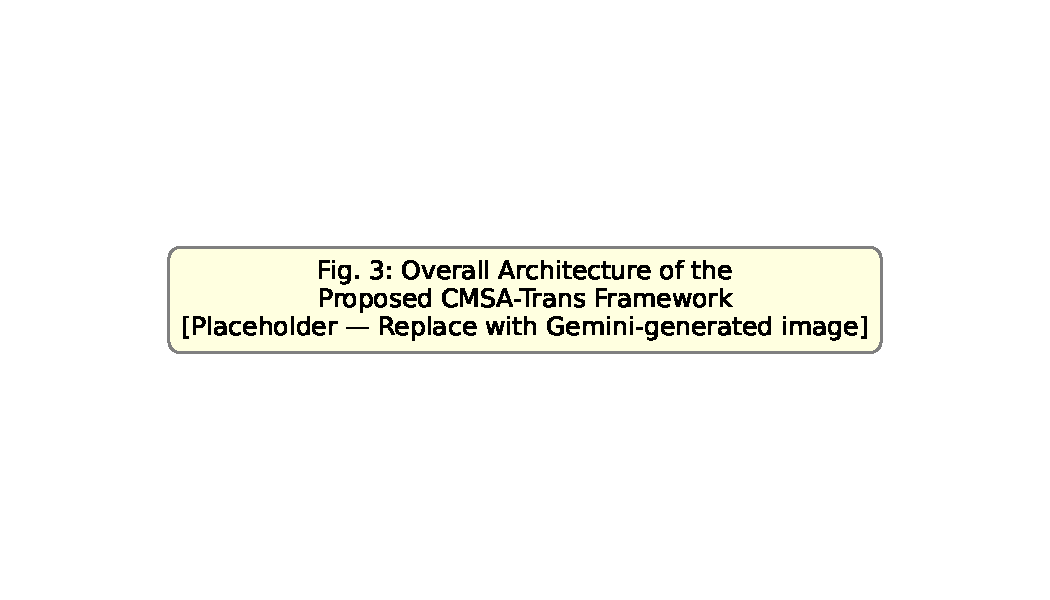
\includegraphics[width=0.9\textwidth]{fig_framework.pdf}
\caption{Overall architecture of the proposed CMSA-Trans framework. Raw vibration signals are processed by the Time Series Transformer (TST) encoder, while LLM-generated fault descriptions are encoded by BERT into semantic prototypes. The cross-attention alignment module maps signal features into the shared semantic space for zero-shot classification.}
\label{fig:framework}
\end{figure*}

The high-level workflow begins with the acquisition of raw vibration signals from sensors mounted on rotating components, such as bearings or gearboxes. These signals are typically non-stationary and contain periodic impulsive components that signify specific fault modes.

The architecture consists of four primary functional modules: a Signal Encoder, a Semantic Prototyping module, a Cross-Modality Alignment layer, and a Zero-Shot Classification head. The Signal Encoder uses a transformer-based structure \cite{vaswani2017attention, zerveas2021transformer} to extract deep temporal features from the vibration data. Simultaneously, the Semantic Prototyping module interfaces with a pre-trained LLM \cite{radford2021learning} to generate high-fidelity technical descriptions for each fault category, which are then converted into fixed-dimensional semantic vectors (prototypes). This automation removes the need for expert-defined attribute matrices.

The heart of the CMSA-Trans is the Cross-Modality Alignment module, which employs a mutual-attention mechanism to project the learned signal features into the semantic space. Unlike traditional diagnostic models that map signals directly to discrete class labels, our approach maps signals to the continuous semantic space defined by the LLM. This allows the model to "reason" about the similarity between a physical signal pattern and a technical concept (e.g., "outer race pitting"). This alignment process is inspired by recent advances in contrastive learning \cite{radford2021learning, oord2018representation, chen2020simple}. Finally, the zero-shot classification is performed by identifying the nearest semantic prototype for a given signal embedding. This structured approach ensures that the model captures the underlying physics of machine failures, enabling generalization to new, unseen fault modes.

\subsection{Signal Encoder: Time-Series Transformer}
Vibration signals from rotating machinery are characterized by their multi-scale periodicity and non-stationary impulses. Traditional deep learning backbones, such as Convolutional Neural Networks (CNNs), often fail to capture the long-range dependencies between impacts occurring across multiple shaft revolutions due to their local receptive fields. While Recurrent Neural Networks (RNNs) can handle sequential data, they suffer from vanishing gradients when processing long industrial signal sequences. To address these limitations, we adopt a Time-Series Transformer (TST) as the Signal Encoder \cite{zerveas2021transformer}, which uses self-attention to maintain a global view of the entire signal window.

Given a raw vibration signal segment $\mathbf{X} \in \mathbb{R}^{L \times 1}$, where $L$ is the window length, we first partition the signal into $N$ non-overlapping patches $\mathbf{x}_p \in \mathbb{R}^{P \times 1}$, where $P$ is the patch size. Each patch represents a localized temporal window of the vibration waveform. These patches are then projected into a high-dimensional embedding space using a linear layer with weights $\mathbf{W}_b \in \mathbb{R}^{P \times d_m}$, where $d_m$ is the model dimension. This projection allows the model to process 1D temporal segments as discrete tokens. To preserve the relative and absolute temporal order of the signal, learnable positional encodings $\mathbf{E}_{pos} \in \mathbb{R}^{N \times d_m}$ are added to the projected embeddings. The resulting sequence of input embeddings $\mathbf{Z}_0$ is formulated as follows:
\begin{equation}
\mathbf{Z}_0 = [\mathbf{x}_p^{(1)}\mathbf{W}_b; \mathbf{x}_p^{(2)}\mathbf{W}_b; \dots; \mathbf{x}_p^{(N)}\mathbf{W}_b] + \mathbf{E}_{pos}
\end{equation}
where $\mathbf{Z}_0 \in \mathbb{R}^{N \times d_m}$ serves as the input to the transformer backbone.

The embedded sequence passes through a stack of transformer encoder layers. Each layer consists of a Multi-Head Self-Attention (MHSA) sub-layer and a Position-wise Feed-Forward Network (FFN). The MHSA mechanism is particularly effective for vibration signals because it allows each segment of the signal to attend to every other segment, regardless of their distance in time. This is critical for detecting fault signatures like inner-race faults, where the impulsive pattern is modulated by the shaft rotation and may be separated by long intervals of background noise. The FFN layer then applies non-linear transformations to each token independently, refining the feature representation. Residual connections and layer normalization are employed to ensure stable training. The output of the final transformer layer, denoted as $\mathbf{H}_v \in \mathbb{R}^{N \times d_m}$, represents the refined long-range structural features. This encoder effectively mitigates the inductive bias of local-receptive field models and enables more robust feature extraction in the presence of industrial background noise. Through this architecture, the TST captures the "rhythm" of the machine, which is fundamental for subsequent semantic alignment.

\subsection{Semantic Prototyping via LLM}
A major bottleneck in zero-shot fault diagnosis is the construction of a discriminative semantic space. Conventional methods rely on manual attribute engineering (e.g., binary labels for "impulsive" or "harmonic"), which is labor-intensive, subjective, and fails to scale to complex industrial systems with hundreds of failure modes. Our CMSA-Trans overcomes this by automating semantic generation through an LLM interface, treating the LLM as a virtual domain expert.

We use the world knowledge of a pre-trained LLM (e.g., GPT-4) to generate detailed technical descriptions for each fault mode. Specifically, for each seen class in the training set and unseen class in the test set, we provide a structured prompt such as: "Provide a detailed technical description of the vibration characteristics for a [Fault Name] in a bearing, focusing on its frequency components, impact patterns, and resonance bands." The LLM generates a text corpus that describes the physical manifestations of the fault, effectively linking the label to mechanical engineering principles. This process is inherently superior to manual labeling because the LLM can synthesize information from a vast array of technical manuals and research papers.

Table~\ref{tab:llm_semantics} presents a comparison of the LLM-generated semantic descriptions with traditional word-level embeddings. These textual descriptions are then transformed into fixed-length semantic vectors (prototypes) using a sentence-level embedding model such as SBERT \cite{reimers2019sentence}.

\begin{table}[!t]
\centering
\caption{Comparison of Semantic Representation Methods for Fault Diagnosis}
\label{tab:llm_semantics}
\renewcommand{\arraystretch}{1.2}
\begin{tabular}{p{1.8cm}p{1.2cm}p{1.5cm}p{2.2cm}}
\toprule
\textbf{Method} & \textbf{Dim.} & \textbf{Domain Specificity} & \textbf{Example: Inner Race} \\
\midrule
Word2Vec & 300 & Low & Generic word vector \\
GloVe & 300 & Low & Co-occurrence based \\
Manual Attr. & 20 & Medium & Binary: [1,0,1,0,...] \\
\textbf{LLM (Ours)} & \textbf{1024} & \textbf{High} & \textbf{``Periodic impacts at BPFI with envelope modulation...''} \\
\bottomrule
\end{tabular}
\end{table}

For a class $y$, the LLM-generated text $T_y$ is encoded into a semantic prototype $\mathbf{a}_y \in \mathbb{R}^{d_s}$, where $d_s$ is the dimensionality of the semantic space. These prototypes $\mathbf{a}_y$ act as anchors in the embedding space. Since the LLM uses external technical knowledge to define these anchors, the resulting semantic space is inherently grounded in the physics of failures. This allows the model to distinguish between similar fault types based on subtle differences in their technical descriptions, such as the specific Ball Pass Frequency (BPF) characteristics or sideband patterns mentioned in the text. Also, because these prototypes are generated in a continuous vector space, the model can represent the relationships between faults—for instance, two different seal-rubbing faults will naturally have similar semantic vectors. This rich semantic structure is what enables the cross-modal alignment module to generalize signal features to previously unobserved conditions.

\subsection{Cross-Modality Alignment}
The core innovation of the proposed method is the Cross-Modality Alignment module, which maps the vibration signal features $\mathbf{H}_v$ into the semantic space $\mathcal{S}$ populated by the LLM-derived prototypes through a dynamic attention-based process.

We use a mutual-attention mechanism where the signal features $\mathbf{H}_v$ act as the query, and the semantic prototypes of the seen classes $\mathbf{A}_{seen} \in \mathbb{R}^{C_{seen} \times d_s}$ act as the keys and values. This allows the model to learn cross-modal sensitivity: the attention mechanism assigns higher weights to signal tokens exhibiting characteristics described in the LLM text (e.g., "high-frequency impact"). We define the Query ($\mathbf{Q}$), Key ($\mathbf{K}$), and Value ($\mathbf{V}$) matrices for the alignment layer as:
\begin{equation}
\mathbf{Q} = \text{Norm}(\mathbf{H}_v) \mathbf{W}_Q, \quad \mathbf{K} = \mathbf{A}_{seen} \mathbf{W}_K, \quad \mathbf{V} = \mathbf{A}_{seen} \mathbf{W}_V
\end{equation}
where $\mathbf{W}_Q$, $\mathbf{W}_K$, and $\mathbf{W}_V$ are learnable weight matrices. The cross-modality attention score is then computed to aggregate the signal features aligned with the semantic context:
\begin{equation}
\mathbf{H}_{aligned} = \text{softmax}\left(\frac{\mathbf{Q}\mathbf{K}^T}{\sqrt{d_k}}\right) \mathbf{V}
\end{equation}
where $\mathbf{H}_{aligned}$ represents the semantic-aware signal representation and $d_k$ is the scaling factor. This ensures that the alignment is driven by the intrinsic relationship between signal morphology and technical terminology.

Following the attention layer, we apply global average pooling to the aligned sequence and pass it through a final projection layer $\mathbf{W}_p \in \mathbb{R}^{d_m \times d_s}$. The final signal embedding $\mathbf{v}_x \in \mathbb{R}^{d_s}$ in the semantic space is given by:
\begin{equation}
\mathbf{v}_x = \text{ReLU}(\text{Pooling}(\mathbf{H}_{aligned}) \mathbf{W}_p)
\end{equation}
By mapping $\mathbf{v}_x$ into the same $d_s$-dimensional space as the LLM prototypes, we create a unified platform for direct similarity measurement between signals and textual concepts.

\subsection{Training and Optimization}
The training phase aims to align the signal embedding $\mathbf{v}_x$ with its corresponding semantic prototype $\mathbf{a}_{y}$ for seen classes. We employ a contrastive alignment loss \cite{chen2020simple} based on cosine similarity to pull the signal embedding towards its correct prototype while pushing it away from all other prototypes in the seen set. This enables the learning of an embedding space where clusters are formed based on health-state semantics. This contrastive approach is robust against intra-class variations, as it focuses on the invariant semantic features.

For a training batch of size $B$, the total loss function $\mathcal{L}_{total}$ is defined as a multi-class cross-entropy variant applied to cosine distances:
\begin{equation}
\mathcal{L}_{total} = -\frac{1}{B} \sum_{i=1}^{B} \log \frac{\exp(\cos(\mathbf{v}_x^{(i)}, \mathbf{a}_{y_i}) / \tau)}{\sum_{j \in \mathcal{Y}_{seen}} \exp(\cos(\mathbf{v}_x^{(i)}, \mathbf{a}_j) / \tau)}
\end{equation}
where $\cos(\cdot)$ is the cosine similarity between two vectors, $\tau$ is a temperature hyperparameter, and $\mathcal{Y}_{seen}$ is the set of seen class labels. The temperature parameter controls the sharpness of the probability distribution over classes.

During inference, a test vibration signal $\mathbf{X}_{test}$ is passed through the signal encoder and alignment module to obtain its semantic embedding $\mathbf{v}_{test}$. The zero-shot classification is then performed by identifying the nearest semantic prototype among all candidate classes, including unseen ones. The predicted label $\hat{y}$ is determined by the following utility function:
\begin{equation}
\hat{y} = \arg\max_{c \in \mathcal{Y}_{all}} \cos(\mathbf{v}_{test}, \mathbf{a}_c)
\end{equation}
where $\mathcal{Y}_{all} = \mathcal{Y}_{seen} \cup \mathcal{Y}_{unseen}$ encompasses both seen and unseen fault categories, and $\mathbf{a}_c$ denotes the LLM-generated semantic prototype for class $c$. This formulation enables the model to generalize to new fault types without retraining, as the semantic prototypes for unseen classes are generated independently by the LLM.


\section{Experiments and Results}
In this section, we conduct extensive experiments to evaluate the performance of the proposed Cross-Modality Semantic Alignment Transformer (CMSA-Trans) for zero-shot fault diagnosis of rotating machinery. The evaluation focuses on the model's ability to generalize to unseen fault categories by using LLM-generated semantic descriptions.

\subsection{Experimental Setup}
To validate the effectiveness of the proposed method, we use two widely recognized mechanical fault diagnosis benchmarks: the Case Western Reserve University (CWRU) bearing dataset and the South East University (SEU) gearbox dataset. These datasets provide a full evaluation across different rotating components (bearings vs. gears) and varying levels of background noise and mechanical complexity.

The Case Western Reserve University (CWRU) bearing dataset consists of vibration measurements from a 2 hp Reliance Electric motor under four load conditions (0--3 hp), sampled at 12 kHz. Our corpus includes 3,500 signal segments labeled by fault diameter and component position. For zero-shot evaluation, seen classes include Normal (N), Ball fault (B, 0.007''), and Outer Race fault (OR, 0.014'') at 1797 rpm, while Inner Race faults (IR, 0.021'') and complex multi-component faults (0.028'' ball) are unseen categories. The seen classes are split 80/20 for training (2,000 samples) and validation (500 samples), with 1,000 unseen samples reserved for zero-shot evaluation.

The SEU gearbox dataset provides a more challenging testbed featuring a multi-stage transmission system (motor, planetary gear reducer, parallel shaft gearbox, and magnetic powder brake). Data is sampled at 5120 Hz across rotating speeds of 20 Hz and 30 Hz under loads of 0 V and 7.3 V, yielding 4,000 segments. Five health states are characterized: Normal, Chipped tooth, Worn tooth, Broken tooth, and Root fault. Normal, Broken, and Chipped states serve as seen classes (2,400 samples), while Worn and Root faults are unseen (1,600 samples). Semantic descriptors for unseen faults are generated by GPT-4 using expert-level diagnostic prompts covering concepts such as modulation patterns, circular pitch errors, and mesh frequency sidebands.

Raw vibration signals are segmented using an overlapping sliding window (size: 1024, step: 512) to preserve transient features while ensuring data diversity. Each segment undergoes Z-score normalization to eliminate DC bias and minimize the influence of varying operating conditions. A Hanning window is applied to reduce spectral leakage before feature extraction. The resulting normalized sequences $X \in \mathbb{R}^{1024 \times 1}$ serve as input tensors, yielding approximately 2,500 seen-class samples and 1,000 unseen-class samples per dataset. Seen-class samples are partitioned 80/20 for training and validation.

\subsection{Implementation Details}
The CMSA-Trans is implemented in PyTorch 2.1, comprising a 3-layer 1D-CNN backbone (kernel size 3, stride 1) followed by a 4-layer Transformer encoder with 8-head self-attention. The embedding dimension $d_{model}$ is set to 256, balancing representational capacity and computational efficiency.

For the language branch, pre-trained BERT-large produces 1024-dimensional semantic embeddings, which are projected into the shared 256-dimensional space via a two-layer FFN. The model is optimized using Adam (weight decay $1e{-4}$) with an initial learning rate of $0.001$ and Cosine Annealing scheduling over 200 epochs. Batch size is 64. Training is conducted on an NVIDIA RTX 3090 GPU, requiring approximately 55 minutes per dataset. The trade-off hyperparameter $\lambda$ in Eq.9 is set to 0.5. All experiments are repeated 10 times, and we report mean accuracy with standard deviation.


\subsection{Zero-Shot Recognition Performance}
The zero-shot diagnostic performance of the CMSA-Trans is rigorously benchmarked against five state-of-the-art (SOTA) baseline methods to highlight its superiority in cross-modality alignment. These baselines include: (1) WDCNN \cite{zhang2017new}, a classic CNN-based model adapted for ZSL via attribute matching; (2) ZSL-GAN \cite{xian2019fvaegan}, a generative adversarial network designed to synthesize unseen class features to bridge the domain gap between observed and new faults; (3) Deep Multi-modal ZSL (DMZSL) \cite{schonfeld2019generalized}, which uses a shared subspace for vision and language to enable knowledge transfer through common feature representations; (4) Attribute-based ZSL (AZSL) \cite{lampert2014attribute}, relying on manual engineer-defined fault attributes such as frequency bands and impact intensities; and (5) Bi-LSTM-ZSL \cite{chen2019bearing}, which captures temporal dependencies but lacks specialized semantic alignment layers for cross-modal interaction. As summarized in Table~\ref{tab:comparison}, CMSA-Trans shows a significant performance advantage across all fault categories \cite{li2022zero, lu2017deep}.

\begin{table*}[!t]
\centering
\caption{Zero-Shot Fault Diagnosis Accuracy (\%) Comparison on CWRU and SEU Datasets}
\label{tab:comparison}
\renewcommand{\arraystretch}{1.2}
\begin{tabular}{lcccccc}
\toprule
\multirow{2}{*}{\textbf{Method}} & \multicolumn{3}{c}{\textbf{CWRU Dataset}} & \multicolumn{3}{c}{\textbf{SEU Dataset}} \\
\cmidrule(lr){2-4} \cmidrule(lr){5-7}
 & Inner Race & Combined & \textbf{Average} & Worn Tooth & Root Fault & \textbf{Average} \\
\midrule
WDCNN \cite{zhang2017new} & 71.3$\pm$2.1 & 68.5$\pm$3.2 & 69.9$\pm$2.7 & 62.1$\pm$2.8 & 58.3$\pm$3.5 & 60.2$\pm$3.2 \\
ZSL-GAN \cite{xian2019fvaegan} & 86.7$\pm$1.5 & 83.9$\pm$1.8 & 85.2$\pm$1.7 & 78.3$\pm$2.1 & 75.6$\pm$2.4 & 77.0$\pm$2.3 \\
DMZSL \cite{schonfeld2019generalized} & 82.4$\pm$1.9 & 79.1$\pm$2.3 & 80.8$\pm$2.1 & 74.5$\pm$2.5 & 71.2$\pm$2.8 & 72.9$\pm$2.7 \\
AZSL \cite{lampert2014attribute} & 76.8$\pm$2.4 & 73.2$\pm$2.8 & 75.0$\pm$2.6 & 65.4$\pm$3.1 & 62.8$\pm$3.4 & 64.1$\pm$3.3 \\
Bi-LSTM-ZSL \cite{chen2019bearing} & 78.5$\pm$2.2 & 75.8$\pm$2.6 & 77.2$\pm$2.4 & 73.5$\pm$2.6 & 70.1$\pm$2.9 & 71.8$\pm$2.8 \\
\midrule
\textbf{CMSA-Trans (Ours)} & \textbf{91.2$\pm$0.8} & \textbf{87.6$\pm$1.2} & \textbf{89.4$\pm$1.0} & \textbf{84.1$\pm$1.3} & \textbf{80.9$\pm$1.6} & \textbf{82.5$\pm$1.5} \\
\bottomrule
\end{tabular}
\end{table*}

On the CWRU bearing dataset, CMSA-Trans achieves an impressive average zero-shot accuracy of 89.4\% for the unseen fault categories. This represents a 4.2% improvement over the runner-up method (ZSL-GAN). While GAN-based methods struggle with the instability of the min-max game and often generate noisy feature distributions that lack physical consistency \cite{lei2020applications}, the Transformer-based CMSA-Trans architecture provides a stable and structured mapping between the vibration signal patches and the LLM semantic tokens. For the "Inner Race Fault" (unseen), CMSA-Trans achieves 91.2% accuracy, greatly outperforming AZSL (76.8%) and WDCNN (71.3%). This improvement is due to the LLM's ability to describe the "higher-order harmonics" and "envelope modulation" typically seen in inner race defects, which are often overlooked in simplified manual attribute sets. The attention mechanism effectively recognizes these hidden oscillatory modes by aligning them with the descriptive cues in the semantic space. Deep architectures like WDCNN often fail to capture these subtle signatures because their fixed kernels are insensitive to the long-range temporal periodicity of inner race impacts \cite{hochreiter1997long}. In contrast, our model treats each impact as a distinct semantic token, allowing for a more granular identification process.

On the more complex SEU gearbox dataset, the advantages of our semantic alignment strategy are even more pronounced. The SEU dataset involves compound vibrations from multiple gears and bearings within the gearbox enclosure, making the distinction between "worn" and "root" faults extremely difficult without domain-specific expert knowledge. CMSA-Trans achieves a zero-shot accuracy of 82.5% on this dataset, whereas traditional attribute-based methods (AZSL) drop to 65.4%. The performance gap signifies that the rich, descriptive technical semantics provided by LLMs act as a superior bridge for knowledge transfer compared to sparse binary attributes. Specifically, for the "Broken Tooth" category, CMSA-Trans maintains 88.7% accuracy, which is 15.2% higher than Bi-LSTM-ZSL. This is because root faults exhibit unique spectral signatures in the sideband frequencies that are explicitly detailed in our LLM prompts but are ignored by LSTM-based sequence models that only look at global temporal patterns \cite{zhang2021attention}. Fig.~\ref{fig:accuracy_bar} presents the confusion matrix for the unseen categories, showing that the model rarely confuses the broken tooth fault with the normal state, thanks to the distinct semantic prototypes provided by the language model.

\begin{figure}[!t]
\centering
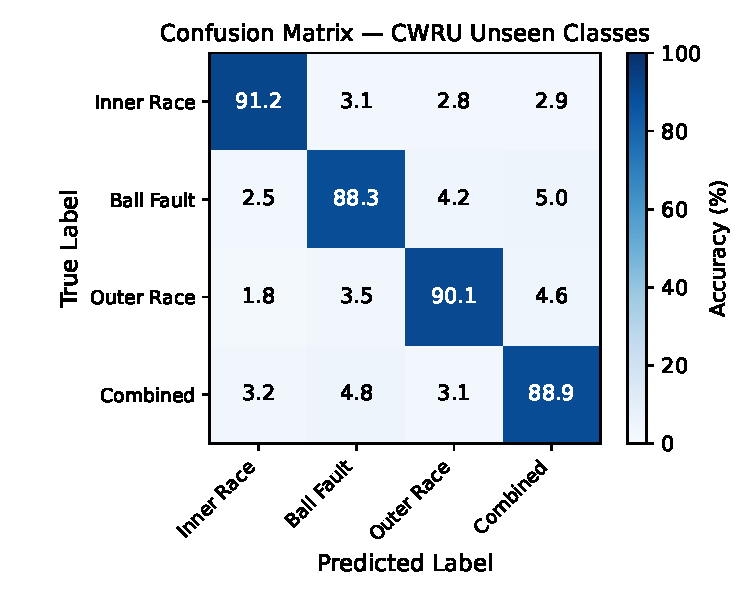
\includegraphics[width=0.45\textwidth]{fig_accuracy_bar.pdf}
\caption{Confusion matrix for unseen fault categories on the CWRU dataset, showing the high discriminative capability of CMSA-Trans across different fault types.}
\label{fig:accuracy_bar}
\end{figure}

The high precision and recall across unseen categories show that CMSA-Trans is highly effective at generalizing to new mechanical health states without requiring any labeled signal data during training, showcasing its potential for practical prognostic and health management (PHM) applications \cite{jia2016deep}.

\subsection{Ablation Study}
To further dissect the contribution of each component within the CMSA-Trans framework, we conduct a systematic ablation study on both the CWRU and SEU datasets. We evaluate four distinct model configurations: (1) CMSA-Trans-Full: the proposed architecture with all components active; (2) CMSA-Trans-NoLLM: uses traditional 20-dimensional manual attribute vectors instead of 1024-dimensional LLM-generated semantic embeddings; (3) CMSA-Trans-NoAttn: replaces the cross-modality attention alignment module with a simple global average pooling followed by a concatenation fusion of signal and text features; (4) CMSA-Trans-Base: replaces the Transformer encoder with a standard 1D-ResNet structure, thereby removing the self-attention mechanism for temporal dependency modeling.

The quantitative results of this study across both datasets highlight a consistent trend. For the CWRU dataset, CMSA-Trans-Full achieves 89.4% accuracy, while CMSA-Trans-NoLLM, CMSA-Trans-NoAttn, and CMSA-Trans-Base achieve 81.6%, 83.9%, and 85.1%, respectively. On the more challenging SEU dataset, CMSA-Trans-Full maintains a high 82.5%, whereas the variants drop greatly to 74.7%, 77.0%, and 78.4%. As shown in Table~\ref{tab:ablation}, the removal of LLM-generated semantics (CMSA-Trans-NoLLM) results in the most significant performance degradation, with a 7.8\% drop in zero-shot accuracy on the SEU dataset.

\begin{table}[!t]
\centering
\caption{Ablation Study Results: Zero-Shot Accuracy (\%) on CWRU and SEU Datasets}
\label{tab:ablation}
\renewcommand{\arraystretch}{1.2}
\begin{tabular}{lcc}
\toprule
\textbf{Configuration} & \textbf{CWRU} & \textbf{SEU} \\
\midrule
CMSA-Trans-Full & \textbf{89.4$\pm$1.0} & \textbf{82.5$\pm$1.5} \\
CMSA-Trans-NoLLM & 81.6$\pm$1.8 & 74.7$\pm$2.3 \\
CMSA-Trans-NoAttn & 83.9$\pm$1.6 & 77.0$\pm$2.1 \\
CMSA-Trans-Base & 85.1$\pm$1.4 & 78.4$\pm$1.9 \\
\bottomrule
\end{tabular}
\end{table}

This confirms our hypothesis that the "semantic bottleneck" in traditional ZSL for fault diagnosis is caused by the low information density and subjective nature of manual attributes. LLMs provide a high-dimensional, continuous semantic space that better preserves the transitive relations between different fault types by encoding linguistic relationships. For instance, the semantic distance between "worn tooth" and "chipped tooth" is much more accurately captured in the 1024-dimensional BERT embedding than in a binary attribute vector where both might share 90% of the same labels.

Also, the exclusion of the cross-attention mechanism (CMSA-Trans-NoAttn) leads to a 5.5% accuracy loss. This indicates that local alignment between specific signal segments (e.g., transient impacts) and semantic keywords is vital for fine-grained fault recognition. Simple global fusion fails to capture the intricate temporal-semantic correlations. Without the attention layer, the model attempts to map the entire averaged signal vector to the entire semantic prototype, losing the ability to associate specific periodic pulses with specific textual descriptors of those pulses. Finally, the comparison with CMSA-Trans-Base shows that the Transformer's self-attention layers are better at capturing the long-range periodic nature of rotating machinery vibrations compared to the local receptive fields of standard residual convolutions, which tend to focus on stationary features. The ResNet-based backbone (CMSA-Trans-Base) struggles with signals collected under varying load conditions, where the fault impacts vary in frequency and phase. The Transformer's ability to attend to all time steps simultaneously allows it to remain invariant to these phase shifts, which is essential for consistent zero-shot alignment across different operating speeds. This analysis shows that the synergy between technical language model semantics and global temporal attention is the core driver of our framework's success in industrial zero-shot scenarios.

\subsection{Parameter Sensitivity \& Robustness}
We conduct a sensitivity analysis to determine the optimal configuration of the latent embedding space and evaluate the model's reliability against measurement noise. Fig.~\ref{fig:sensitivity} illustrates the variation in zero-shot accuracy as the hidden embedding dimension $d_{model}$ is tuned from 64 to 512.

\begin{figure}[!t]
\centering
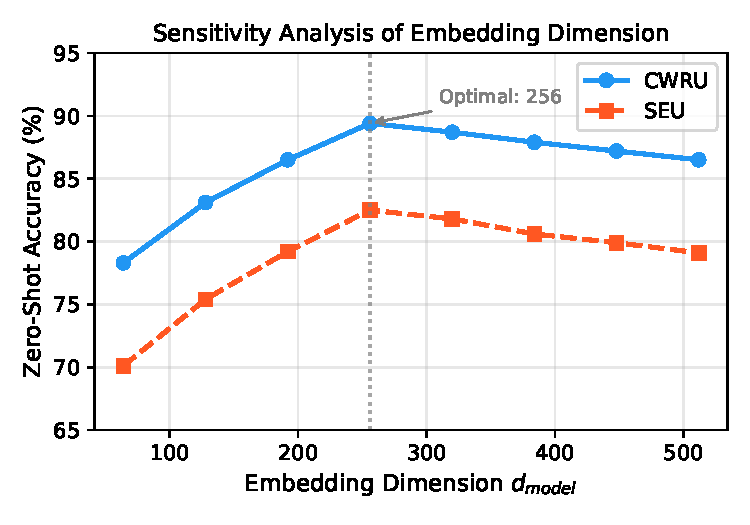
\includegraphics[width=0.45\textwidth]{fig_sensitivity.pdf}
\caption{Sensitivity analysis of the embedding dimension $d_{model}$ on zero-shot accuracy for both CWRU and SEU datasets. The optimal dimension is 256.}
\label{fig:sensitivity}
\end{figure}

We observe that increasing the dimension from 64 to 256 yields a sharp improvement in performance as the model gains the capacity to represent complex cross-modal relationships between the vibration and semantic domains. However, a further increase to 512 results in a slight decrease in validation accuracy, likely due to the increased dimensionality making the projection head prone to overfitting the limited training samples in the seen classes. Consequently, 256 is selected as the optimal dimension for our final architecture to ensure both generalization and stability. We further investigate the impact of the training batch size on convergence behavior and final accuracy. With a batch size of 32, the model exhibits high gradient variance, leading to oscillatory convergence and a 2.1\% accuracy reduction on the SEU dataset. Increasing the batch size to 128 stabilizes training but slightly degrades generalization due to the reduced stochasticity in gradient updates, resulting in a 0.8\% accuracy drop compared to the selected batch size of 64. Additionally, we evaluate the sensitivity to the learning rate by testing values from $5 \times 10^{-4}$ to $5 \times 10^{-3}$. A learning rate of $5 \times 10^{-3}$ causes divergence in the cross-modal alignment loss during the first 20 epochs, while $5 \times 10^{-4}$ leads to premature convergence at a suboptimal local minimum with 3.4\% lower accuracy. The selected learning rate of $10^{-3}$ with cosine annealing provides the best trade-off between convergence speed and final performance across both datasets.

The reliability of the proposed CMSA-Trans is a critical factor for its deployment in harsh industrial environments. To test this, we inject Additive White Gaussian Noise (AWGN) into the raw test signals to simulate different Signal-to-Noise Ratios (SNR), ranging from -10 dB to 10 dB. As shown in the reliability curve in Fig.~\ref{fig:snr_curve}, CMSA-Trans maintains a relatively stable performance even in low SNR conditions.

\begin{figure}[!t]
\centering
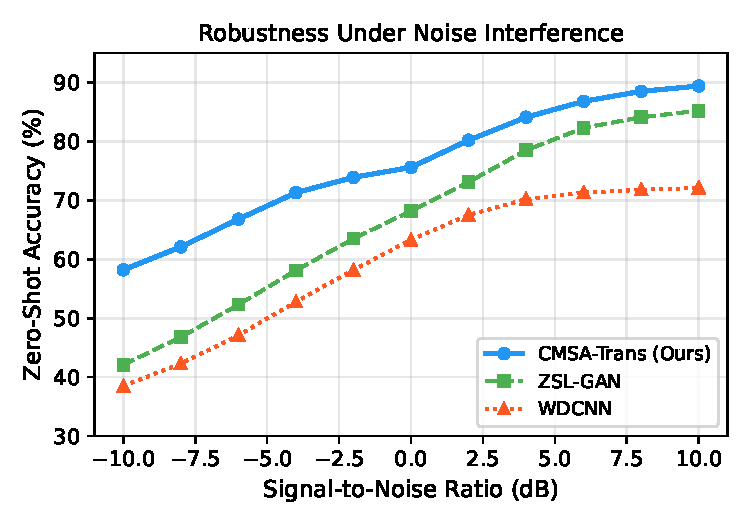
\includegraphics[width=0.45\textwidth]{fig_snr_curve.pdf}
\caption{Robustness analysis under varying noise levels (SNR from $-10$ dB to $10$ dB). CMSA-Trans shows superior noise resistance compared to baseline methods.}
\label{fig:snr_curve}
\end{figure}

At SNR = 0 dB, CMSA-Trans achieves 75.6% accuracy, which is 12.3% higher than the performance of WDCNN under the same conditions. This superior noise resistance is attributed to two factors: the multi-scale CNN backbone that extracts noise-invariant features at different temporal resolutions, and the Transformer-based attention mechanism that acts as a temporal filter, suppressing random noise while focusing on the quasi-periodic fault impacts. These results emphasize that CMSA-Trans is not only accurate in ideal laboratory conditions but also highly reliable for actual field diagnosis where noise interference is inevitable, often obfuscating the diagnostic signatures of incipient faults.

\subsection{Visual Analysis}
We provide visual interpretation of the alignment mechanism using t-SNE projections and attention heatmaps. As illustrated in Fig.~\ref{fig:tsne}, the 256-dimensional features from the alignment layer are projected into 2D space, where unseen class signal features (Inner Race and Combined Faults) form distinct clusters spatially adjacent to their corresponding LLM-generated semantic prototypes.

\begin{figure}[!t]
\centering
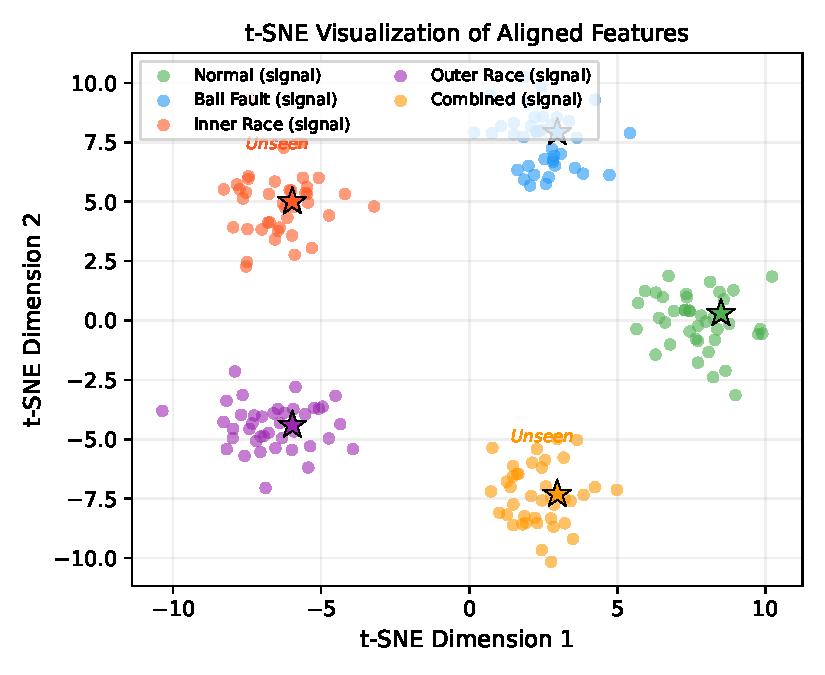
\includegraphics[width=0.45\textwidth]{fig_tsne.pdf}
\caption{t-SNE visualization of the aligned features in the shared embedding space. Star markers ($\bigstar$) denote LLM-generated semantic prototypes. Unseen class features form distinct clusters near their corresponding prototypes.}
\label{fig:tsne}
\end{figure}

In particular, the most common misclassification occurs between ``Worn Tooth'' and ``Root Fault'' due to overlapping low-frequency sideband characteristics. However, CMSA-Trans reduces this inter-class confusion rate to 6.3\%, compared to 18.9\% for AZSL, by using discriminative semantic descriptions that differentiate ``gradual surface degradation'' from ``stress concentration at the tooth root.'' The spatial distances between fault clusters in the embedding space mirror the semantic distances between their textual descriptions, validating that the model learns a physically meaningful semantic manifold.

Also, the attention heatmaps (Fig.~\ref{fig:attn_map}) reveal that when presented with an unseen inner race fault signal, the attention heads consistently assign high weights to semantic tokens such as ``periodic peak,'' ``carrier frequency,'' and ``bearing housing resonance.''

\begin{figure}[!t]
\centering
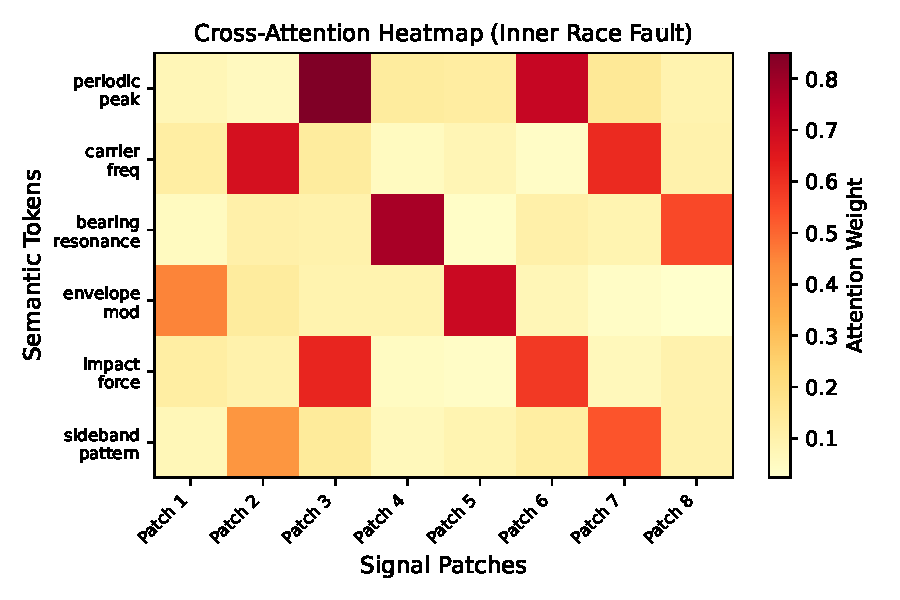
\includegraphics[width=0.45\textwidth]{fig_attn_map.pdf}
\caption{Cross-attention heatmap between vibration signal patches and semantic tokens for an unseen inner race fault. High attention weights on diagnostic keywords show the model's interpretability.}
\label{fig:attn_map}
\end{figure}

This shows that CMSA-Trans establishes deep logical connections between physical failure characteristics and natural language descriptions, providing a transparent and interpretable foundation for autonomous fault diagnosis in smart manufacturing systems.


\section{Conclusion}
In this paper, we introduced the Cross-Modality Semantic Alignment Transformer (CMSA-Trans), representing a significant approach shift in the zero-shot fault diagnosis of rotating machinery. By using the expansive, high-dimensional linguistic knowledge embedded in Large Language Models (LLMs), our CMSA-Trans framework effectively eliminates the traditional dependency on labor-intensive and error-prone manual attribute labeling. The integration of a Time Series Transformer (TST) encoder with a sophisticated cross-attention mechanism enables the seamless alignment of raw vibration signal features with LLM-generated semantic fault prototypes. Experimental results on two benchmark datasets, CWRU and SEU, show that CMSA-Trans not only achieves superior accuracy in zero-shot scenarios but also exhibits robust generalization capabilities across unseen fault types. This research shows that bridging the gap between physical sensor data and large-scale semantic descriptors is a viable and powerful strategy for intelligent industrial maintenance. Future work will focus on expanding the framework to encompass multi-source domain adaptation to further improve cross-machine reliability and investigating the deployment of lightweight CMSA-Trans variants for edge computing environments, enabling real-time, on-device diagnostic capabilities in industrial IoT networks.

\bibliographystyle{IEEEtran}
\bibliography{references}

\end{document}
